\chapter{- Further technical drawings}
\label{sec:a-techDraw}

\section{Raspberry Pi B+}
\label{sec:goals:rpib}
\begin{figure}[H]
    \centering
    
\includegraphics[angle=90,width=0.75\textwidth]{fig/ch-zz-appendix/A-techDraw/A4_tech_draw_topview_rpi}
    \caption{Technical drawing of Raspberry Pi B+ (topview)}
    \label{fig:parts:rpi_topview}
\end{figure}

\newpage
\section{Adafruit GPS Hat}
\label{sec:goals:gpshat}
\begin{figure}[H]
    \centering
    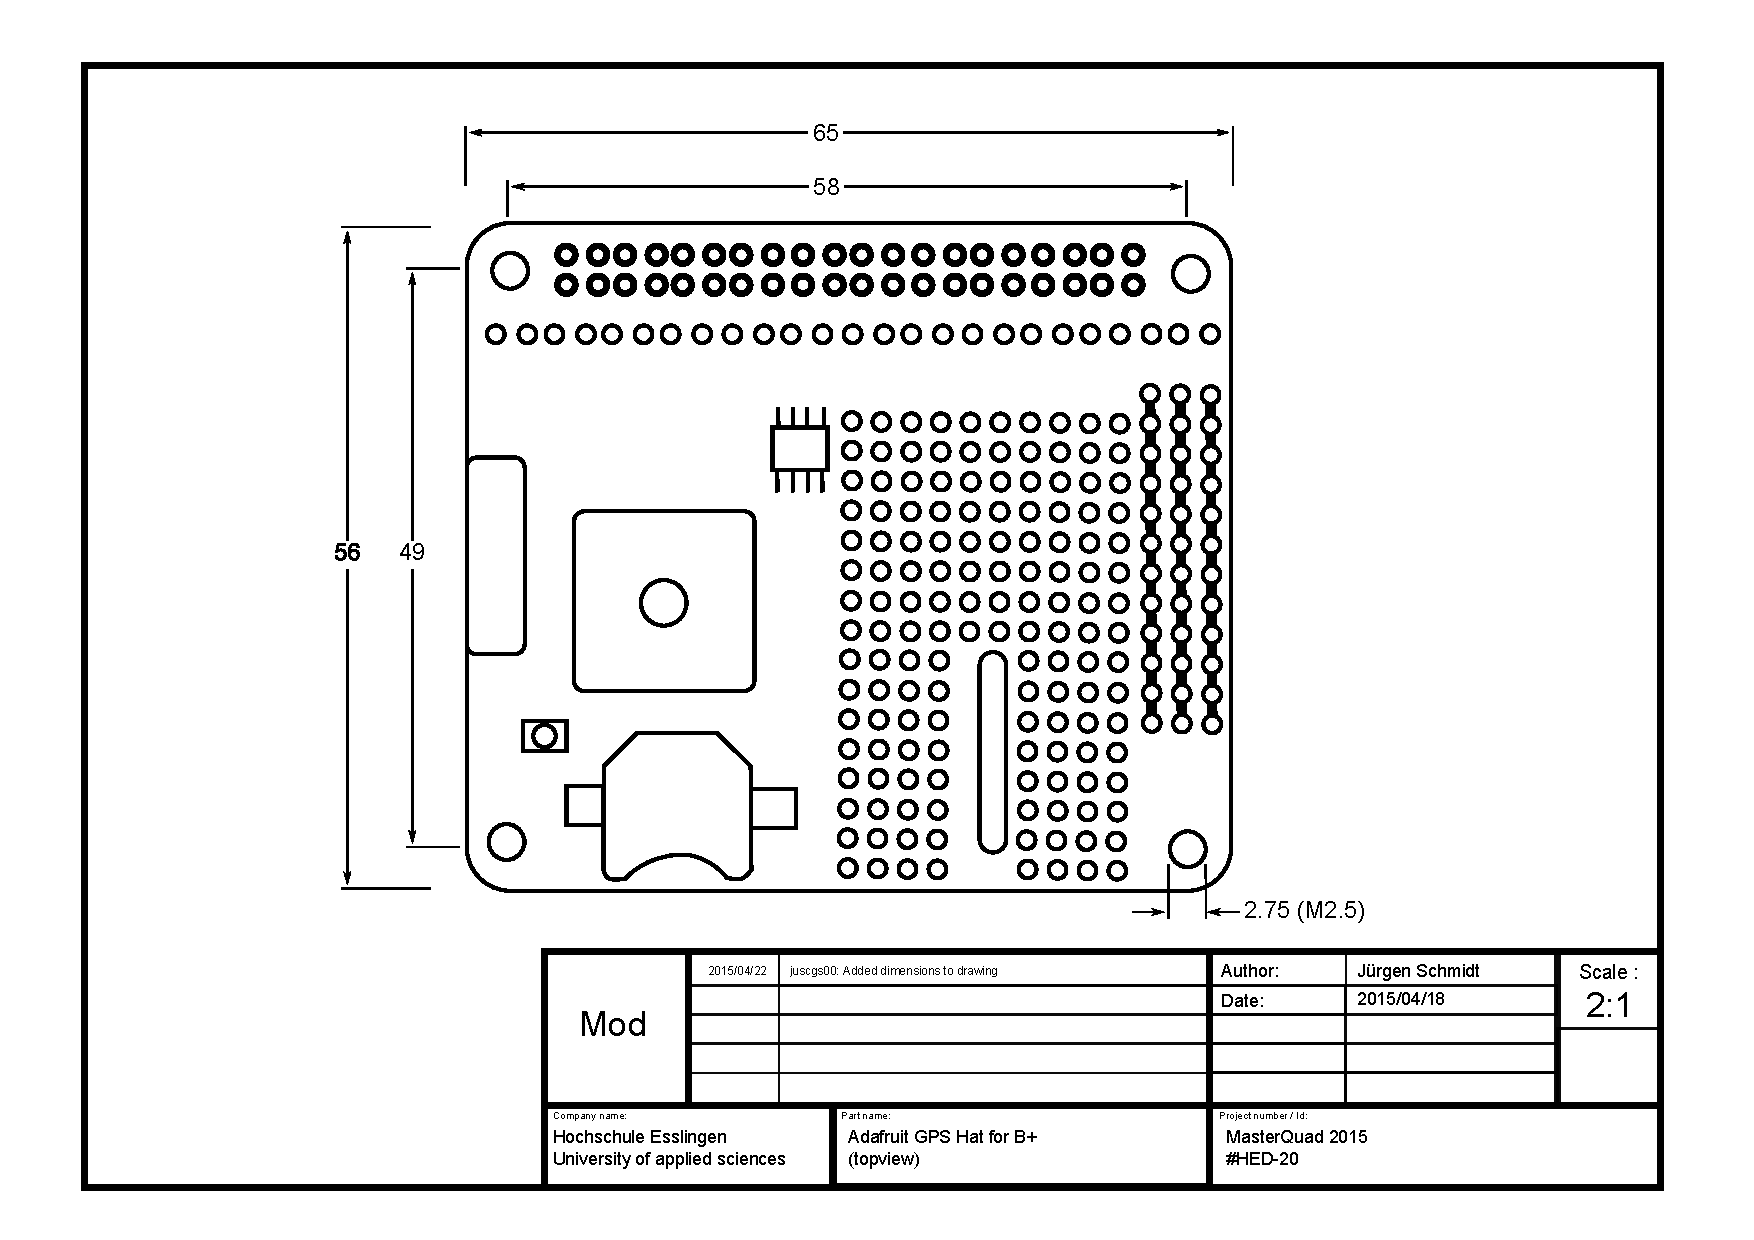
\includegraphics[angle=90,width=0.88\textwidth]{fig/ch-zz-appendix/A-techDraw/A4_tech_draw_topview_gpshat}
    \caption{Technical drawing of Adafruit GPS Hat}
    \label{fig:parts:gps_topview}
\end{figure}

\newpage
\section{Polulu AltIMU v4}
\label{sec:goals:altimu}
\begin{figure}[H]
    \centering
    
\includegraphics[angle=90,width=0.88\textwidth]{fig/ch-zz-appendix/A-techDraw/A4_tech_draw_topview_imu}
    \caption{Technical drawing of Polulu AltIMU v4}
    \label{fig:parts:imu_topview}
\end{figure}

%\newpage
\section{Adafruit 12bit ADC over I2C}
\label{sec:goals:adc}
\begin{figure}[H]
    \centering
    
\includegraphics[angle=90,width=0.88\textwidth]{fig/ch-zz-appendix/A-techDraw/A4_tech_draw_topview_adc}
    \caption{Technical drawing of Adafruit 12bit ADC over I2C}
    \label{fig:parts:adc_topview}
\end{figure}

\chapter{- Code documentation}
\label{sec:b-codeDoc}

For the full code documentation please see Doxygen's HTML output at the SVN repository at
\texttt{/impl/trunk/doc/html/index.html}

The HTML output looks like the following exemplary screen capture in figure \ref{fig:b-codeDoc:doxygenBrowser}.

\begin{figure}[h]
    \centering
    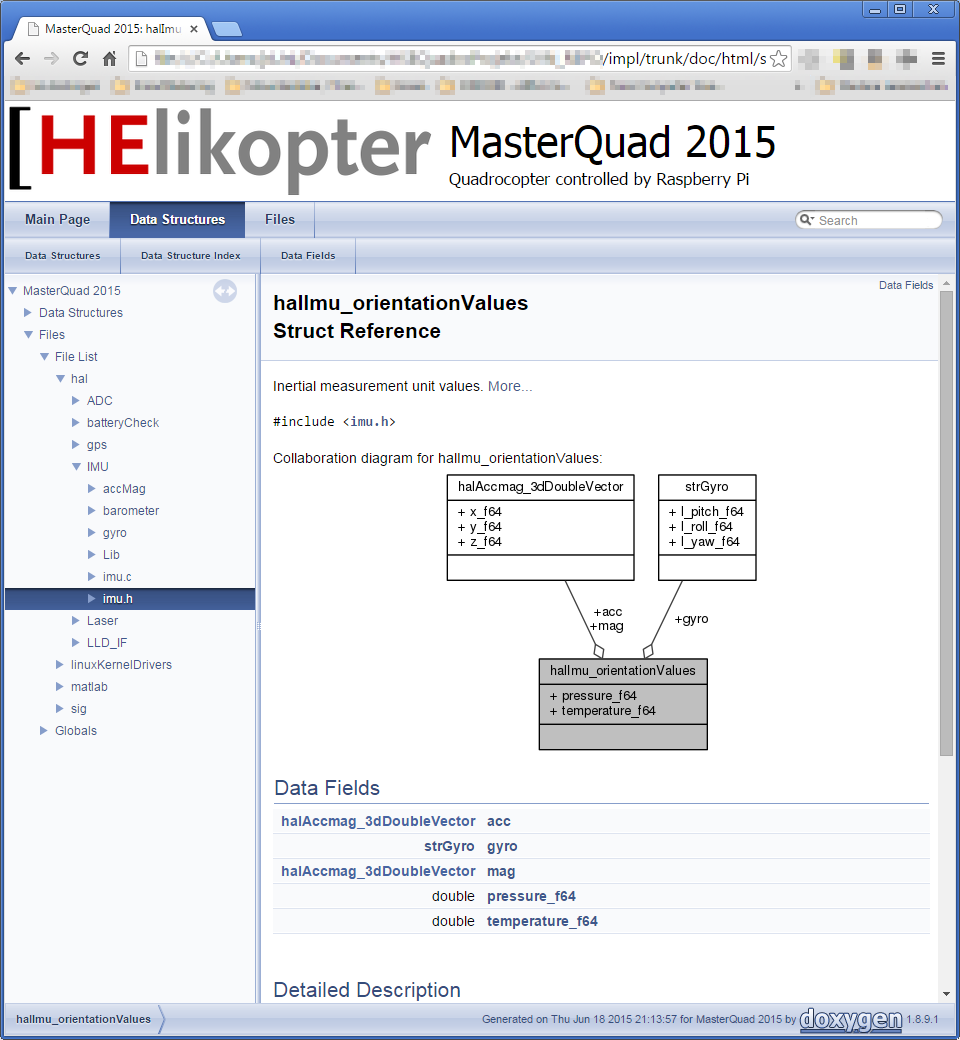
\includegraphics[width=0.86\textwidth]{fig/ch-zz-appendix/B-code-documentation/doxygenHtmlScreen}
    \caption{Screen capture of Doxygen's HTML output for code documentation}
    \label{fig:b-codeDoc:doxygenBrowser}
\end{figure}

\chapter{- Soure code}
\label{sec:append-sourceCode}

\section{S-Function Builder generated C-Code}
\label{sec:c-sFunc-Code}

\subsection{Raw C-Code template of S-Function}
\label{sec:c-sFunc-Code:rawTemplate}
\begin{lstlisting}[caption={[C-Code template 'myUdpSource.c' generated by the S-Function Builder]Complete C-Code template file 'myUdpSource.c' generated by the S-Function Builder according to the example shown in chapter \ref{sec:udpMatlab:simulinkBlock:builder}},label=code:c-sFunc-Code:rawTemplate]
\end{lstlisting}

\newpage
\subsection{Raw template code of wrapper function}
\label{sec:c-sFunc-Code:wrapperOutputs}


\section{MATLAB-Code for Simulink 3D visualization}
\label{sec:d-mFunc-Code}

\begin{lstlisting}[caption={[MATLAB-Code for 3D visualization of orientation angles]MATLAB-Code for a MATLAB-function block to realize a 3D visualization of the Quadrocopter's orientation angles},language=MATLAB,label=code:d-mFunc-Code:3dViz]
\end{lstlisting}

\section{Kernel driver \texttt{ppmDemux}}
\label{sec:append-ppmDemuxCode}

\begin{lstlisting}[caption={[Source code listing of ppmDemux.c]Complete soure code of the proof-of-concept kernel driver \texttt{ppmDemux} to measure the time between to rising edges of GPIO pin 24.},label=code:append-ppmDemuxCode:ppmDemux]
#include <linux/module.h>
#include <linux/fs.h>
#include <linux/cdev.h>
#include <linux/device.h>
#include <linux/gpio.h>
#include <asm/uaccess.h>
#include <linux/interrupt.h>
#include <linux/sched.h>

#include <linux/init.h>
#include <linux/kernel.h>
#include <linux/errno.h>
#include <linux/fs.h>
#include <linux/uaccess.h>
#include <linux/io.h>

#include <asm-generic/errno-base.h>
#include <linux/wait.h>

/*
 * System Timer base address
 *
 * Note: Phys. SoC address 0x7Ennnnnn (as given in data sheet) gets mapped
 *       to 0x20nnnnnn by built-in MMU
 *
 * */
#define TIMER_PAGE_BASE 0x20003000
#define TIMER_OFFSET 	4

#define M_GPIO_NUMBER	24

static dev_t gpio_dev_number;
static struct cdev *driver_object;
static struct class *gpio_class;
static struct device *gpio_dev;
static int rpi_irq_17;
static char *devname = "ppmDemux";
static wait_queue_head_t sleeping_for_ir;

static void *timer_pf;        /* the page frame containing the timer */
static unsigned long *timer_low;
static unsigned long *timer_high;

struct timedInterrupt{
	int 					irqNum;
	unsigned long	timer_l;
	unsigned long	timer_h;
};

static struct timedInterrupt modIrqObj;

static irqreturn_t rpi_gpio_isr( int irq, void *data )
{
	/* wake up read function to retrieve new data */
	wake_up( &sleeping_for_ir );

	return IRQ_HANDLED;
}

static irqreturn_t hard_isr( int irq, void *dev_id )
{
	/* read free running timer (64bit) @ 1MHz */
	modIrqObj.timer_l = readl(timer_low);
	modIrqObj.timer_h = readl(timer_high);

	/* counts rising edges since last read */
	modIrqObj.irqNum += 1;

	return IRQ_WAKE_THREAD;
}

static int config_gpio( int gpionr )
{
	int err, rpi_irq;
	char name[20];

	snprintf( name, sizeof(name), "rpi-gpio-%d", gpionr );
	err = gpio_request( gpionr, name );
	if (err) {
		printk("gpio_request failed %d\n", err);
		return -1;
	}
	err = gpio_direction_input( gpionr );
	if (err) {
		printk("gpio_direction_input failed %d\n", err);
		gpio_free( gpionr );
		return -1;
	}
	rpi_irq = gpio_to_irq( gpionr );
	printk("gpio_to_irq returned %d\n", rpi_irq);
	if (rpi_irq < 0) {
		printk("gpio_to_irq failed %d\n", rpi_irq);
		gpio_free( gpionr );
		return -1;
	}
	err = request_threaded_irq( rpi_irq, hard_isr, rpi_gpio_isr, IRQF_TRIGGER_RISING, devname, driver_object);
	printk("driver_object: %p\n", driver_object);
	if (err) {
		printk("request_irq failed with %d\n", err);
		gpio_free( gpionr );
		return -1;
	}
	printk("gpio %d successfull configured\n", gpionr);
	return rpi_irq;
}

static ssize_t driver_read( struct file *instanz, char __user *user,
		size_t count, loff_t *offset )
{
	unsigned long not_copied, to_copy;

	/* re-init data structure */
	modIrqObj.irqNum 	= 0;
	modIrqObj.timer_l	= 0;
	modIrqObj.timer_h	= 0;

	/* wait for an rising edge event (caught by ISR) */
	wait_event_interruptible( sleeping_for_ir, modIrqObj.irqNum);

	/* copy data to user-sapce */
	to_copy = min( count, sizeof(modIrqObj) );
	not_copied = copy_to_user(user, &(modIrqObj), to_copy);

	return to_copy-not_copied;
}

static struct file_operations fops = {
		.owner= THIS_MODULE,
		.read= driver_read,
};

static int __init mod_init( void )
{
	dev_info(gpio_dev, "mod_init");
	init_waitqueue_head( &sleeping_for_ir );

	if( alloc_chrdev_region(&gpio_dev_number,0,1,"gpioirq24")<0 )
		return -EIO;

	driver_object = cdev_alloc(); /* Anmeldeobjekt reservieren */

	if( driver_object==NULL )
		goto free_device_number;

	driver_object->owner = THIS_MODULE;
	driver_object->ops = &fops;

	if( cdev_add(driver_object,gpio_dev_number,1) )
		goto free_cdev;

	gpio_class = class_create( THIS_MODULE, "gpioirq24" );

	if( IS_ERR( gpio_class ) ) {
		pr_err( "gpioirq17: no udev support\n");
		goto free_cdev;
	}
	gpio_dev = device_create( gpio_class, NULL, gpio_dev_number, NULL, "%s", "gpioirq24" );

	if ( IS_ERR(gpio_dev) )
		goto free_class;

	rpi_irq_17 = config_gpio( M_GPIO_NUMBER );
	if (rpi_irq_17 < 0) {
		goto free_device;
	}

	/* get the mapping for the page frame containing the timer */
	timer_pf = ioremap(TIMER_PAGE_BASE, SZ_4K);
	/* and set the pointer to the timer itself */
	timer_low = (unsigned long*)(timer_pf + TIMER_OFFSET);
	timer_high = (unsigned long*)(timer_pf + TIMER_OFFSET + TIMER_OFFSET);
	pr_info("bcm2708_usec initialized; timer @ %pK\n", timer_low);

	return 0;

	/* ERROR HANDLING (below) */
	free_device:
	device_destroy( gpio_class, gpio_dev_number );
	free_class:
	class_destroy( gpio_class );
	free_cdev:
	kobject_put( &driver_object->kobj );
	free_device_number:
	unregister_chrdev_region( gpio_dev_number, 1 );
	/* if the timer was mapped (final step of successful module init) */
	if (timer_pf)
		/* release the mapping */
		iounmap(timer_pf);
	return -EIO;
}

static void __exit mod_exit( void )
{
	/* if the timer was mapped (final step of successful module init) */
	if (timer_pf)
		/* release the mapping */
		iounmap(timer_pf);

	dev_info(gpio_dev, "mod_exit");
	device_destroy( gpio_class, gpio_dev_number );
	class_destroy( gpio_class );
	cdev_del( driver_object );
	unregister_chrdev_region( gpio_dev_number, 1 );
	free_irq(rpi_irq_17, driver_object);
	gpio_free( M_GPIO_NUMBER );
	return;
}

module_init( mod_init );
module_exit( mod_exit );
MODULE_LICENSE("GPL");
\end{lstlisting}

\begin{lstlisting}[caption={[Source code listing of getPpmDemuxValues.c]Complete soure code of the test file \texttt{getPpmDemuxValues.c} to read the output of the proof-of-concept kernel driver \texttt{ppmDemux}.},label=code:append-ppmDemuxCode:ppmDemusReader]
#include <stdio.h>
#include <fcntl.h>

int main( int argc, char **argv, char **envp )
{
    int fd;

    /* structured data received from kernel driver output */
    struct outputStruct{
        int 					irqNum;
        unsigned long timer_l;
        unsigned long timer_h;
    };

    struct outputStruct localOutputBlock;
    
    unsigned long long newTime = 0;
    unsigned long long oldTime = 0;

    /* open character file handler of kernel driver ppmDemux */    
    fd = open( "/dev/gpioirq24", O_RDONLY );
    if (fd<0) {
        perror("/dev/gpioirq24");
        return -1;
    }

    while (1) {
        unsigned long recvBytes=0;

	/* evaluate only lower part of counter value (wrap around every 
	 * ~4.2 seconds is sufficient for this testing approach) 
	 */
        recvBytes = read( fd, 
													&(localOutputBlock), 
													sizeof(struct outputStruct) );
        newTime = (unsigned long long)localOutputBlock.timer_l; 
        printf("interrupts: %d, delta: %llu us\n",
								localOutputBlock.irqNum, 
								newTime - oldTime );

        oldTime = newTime;
    }
    return 0;
}

\end{lstlisting}

\chapter{- Default login credentials}
\label{sec:d-credentials}

\section{Development Environment}
\label{sec:d-credentials:vm}
\textbf{User:} \texttt{user}\\
\textbf{Password:} \texttt{user}

\section{Raspberry Pi Firmware}
\label{sec:d-credentials:rpi}
\textbf{User:} \texttt{pi}\\
\textbf{Password:} \texttt{raspberry}

\textbf{User:} \texttt{root}\\
\textbf{Password:} \texttt{raspberry}
